
\begin{figure}[t!]
    \centering
    \vspace{-2em}
    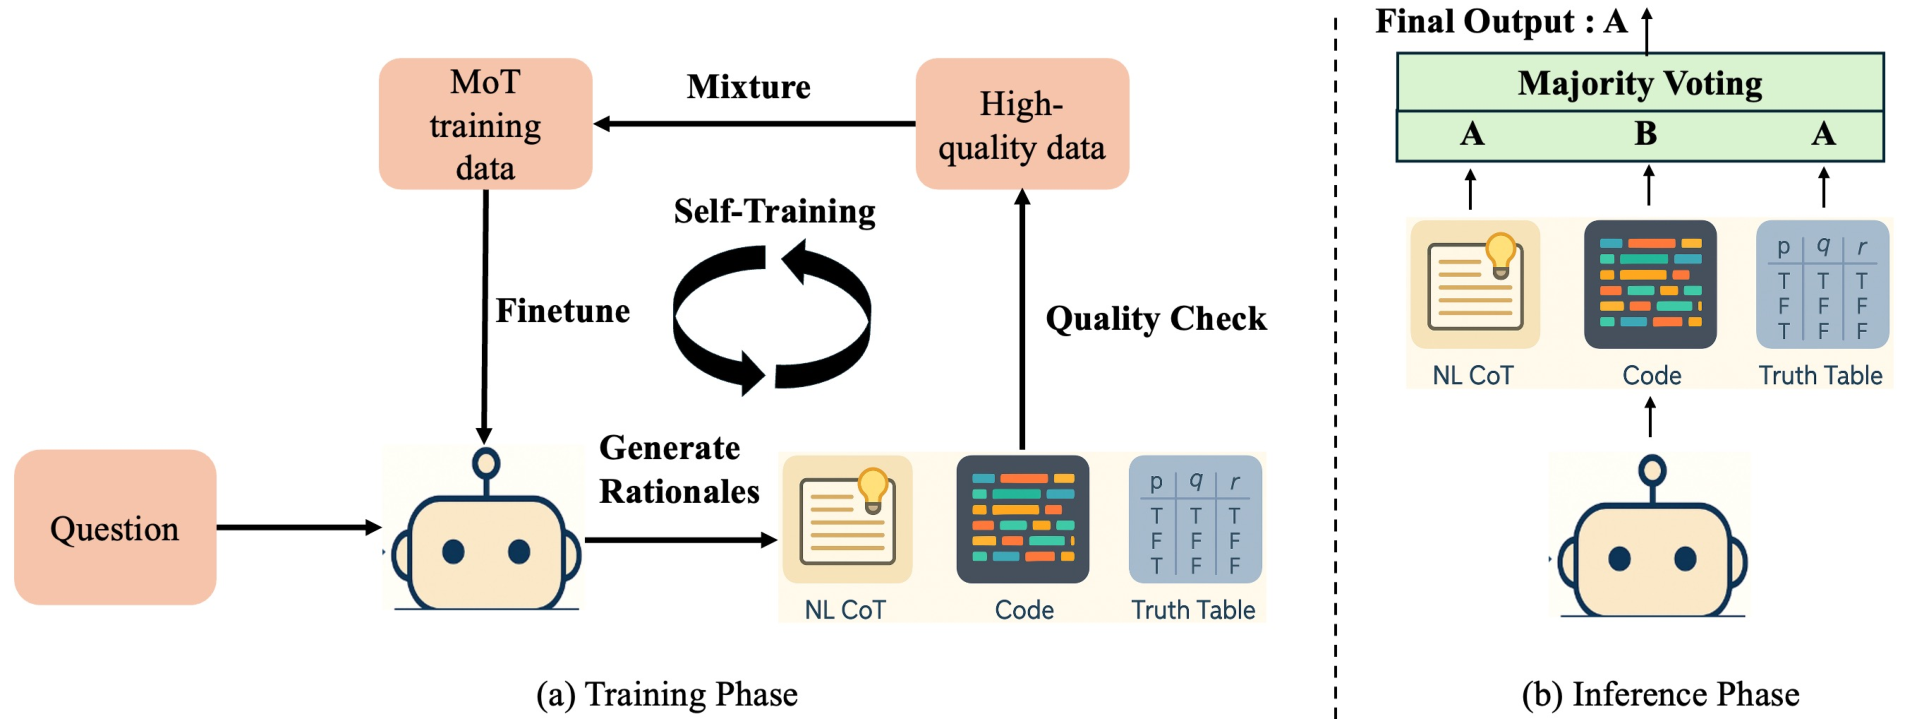
\includegraphics[width=0.85\linewidth]{Figure/raw_figure/MoT_Pipeline.pdf}
    \caption{\footnotesize{Illustration of our MoT Framework. (a) \textbf{Training phase} with three key steps: 1) \textbf{Rationale Generation} where given an initial seed dataset, LLM generates rationales across reasoning modalities (NL, Code, and Truth Table); 2) \textbf{Quality Checking and Merging} where generated rationales are checked for correctness and format consistency, then merged into high-quality MoT training data; and 3) \textbf{Finetuning} where the model is trained using the MoT data. These steps iteratively repeats, forming a self-evolving training cycle. (b) \textbf{Inference phase:} the trained model generates outputs for each reasoning modality and applies majority voting to yield the final prediction (e.g., A).
}}
    \label{fig:pipeline}
\vspace{-1em}
\end{figure}